\begin{figure*}[t]
\centering
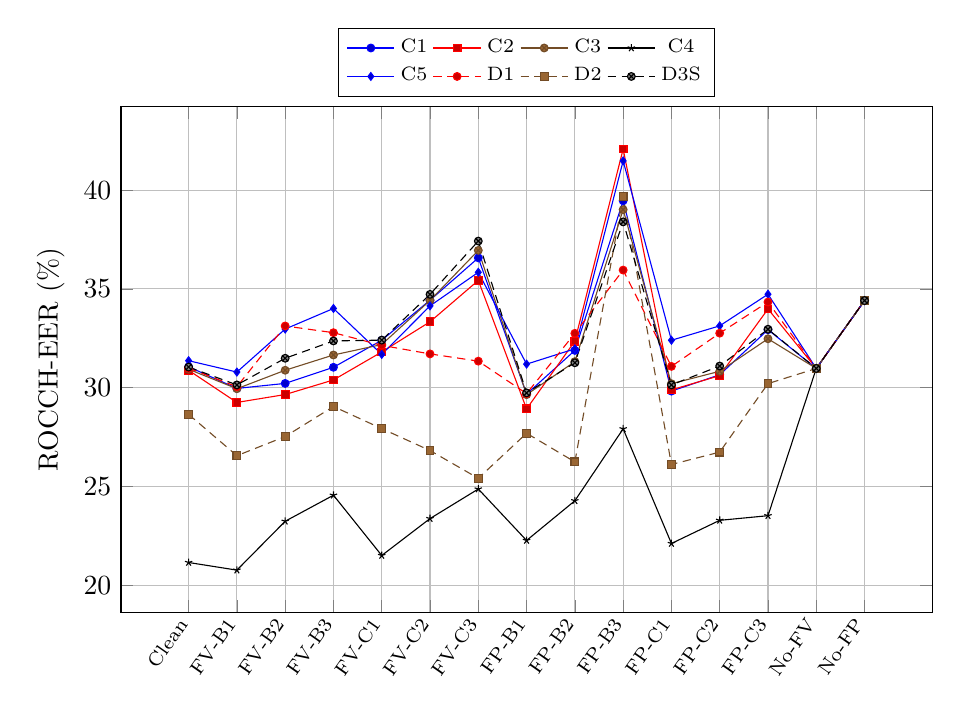
\begin{tikzpicture}
\begin{axis}[width=0.98\textwidth,height=8cm,ylabel={ROCCH-EER (\%)},symbolic x coords={Clean,FV-B1,FV-B2,FV-B3,FV-C1,FV-C2,FV-C3,FP-B1,FP-B2,FP-B3,FP-C1,FP-C2,FP-C3,No-FV,No-FP},xtick=data,x tick label style={rotate=55,anchor=east,font=\scriptsize},legend columns=4,legend style={at={(0.5,1.02)},anchor=south,font=\scriptsize},grid=major,mark size=1.4pt]
\addplot coordinates {(Clean,31.053879) (FV-B1,29.960018) (FV-B2,30.212777) (FV-B3,31.029605) (FV-C1,32.397720) (FV-C2,34.425000) (FV-C3,36.568695) (FP-B1,29.670781) (FP-B2,31.883612) (FP-B3,39.461538) (FP-C1,29.823362) (FP-C2,30.649566) (FP-C3,32.931398) (No-FV,30.969136) (No-FP,34.406793)};
\addlegendentry{C1}
\addplot coordinates {(Clean,30.876043) (FV-B1,29.250000) (FV-B2,29.649671) (FV-B3,30.388634) (FV-C1,31.804301) (FV-C2,33.332711) (FV-C3,35.426606) (FP-B1,28.922035) (FP-B2,32.352636) (FP-B3,42.080590) (FP-C1,29.886354) (FP-C2,30.606757) (FP-C3,33.980130) (No-FV,30.969136) (No-FP,34.406793)};
\addlegendentry{C2}
\addplot coordinates {(Clean,30.928887) (FV-B1,29.943925) (FV-B2,30.880000) (FV-B3,31.651703) (FV-C1,32.181934) (FV-C2,34.414088) (FV-C3,36.946803) (FP-B1,29.644362) (FP-B2,31.315500) (FP-B3,39.010761) (FP-C1,30.198800) (FP-C2,30.827131) (FP-C3,32.472661) (No-FV,30.969136) (No-FP,34.406793)};
\addlegendentry{C3}
\addplot coordinates {(Clean,21.146749) (FV-B1,20.759950) (FV-B2,23.234456) (FV-B3,24.553130) (FV-C1,21.501866) (FV-C2,23.370130) (FV-C3,24.867347) (FP-B1,22.262861) (FP-B2,24.272131) (FP-B3,27.913994) (FP-C1,22.109799) (FP-C2,23.281337) (FP-C3,23.515957) (No-FV,30.969136) (No-FP,34.406793)};
\addlegendentry{C4}
\addplot coordinates {(Clean,31.362543) (FV-B1,30.786874) (FV-B2,32.965116) (FV-B3,34.006444) (FV-C1,31.679598) (FV-C2,34.137066) (FV-C3,35.838422) (FP-B1,31.189003) (FP-B2,31.963872) (FP-B3,41.478361) (FP-C1,32.397297) (FP-C2,33.126284) (FP-C3,34.727525) (No-FV,30.969136) (No-FP,34.406793)};
\addlegendentry{C5}
\addplot coordinates {(Clean,30.983505) (FV-B1,30.045802) (FV-B2,33.120038) (FV-B3,32.780612) (FV-C1,32.138776) (FV-C2,31.706738) (FV-C3,31.340474) (FP-B1,29.696970) (FP-B2,32.748349) (FP-B3,35.950374) (FP-C1,31.074054) (FP-C2,32.756329) (FP-C3,34.333406) (No-FV,30.969136) (No-FP,34.406793)};
\addlegendentry{D1}
\addplot coordinates {(Clean,28.645278) (FV-B1,26.553756) (FV-B2,27.523055) (FV-B3,29.043707) (FV-C1,27.924855) (FV-C2,26.815068) (FV-C3,25.408213) (FP-B1,27.690174) (FP-B2,26.238938) (FP-B3,39.675145) (FP-C1,26.107994) (FP-C2,26.735614) (FP-C3,30.203849) (No-FV,30.969136) (No-FP,34.406793)};
\addlegendentry{D2}
\addplot coordinates {(Clean,31.040809) (FV-B1,30.136111) (FV-B2,31.486081) (FV-B3,32.362559) (FV-C1,32.404762) (FV-C2,34.721342) (FV-C3,37.418704) (FP-B1,29.732789) (FP-B2,31.256983) (FP-B3,38.391185) (FP-C1,30.137342) (FP-C2,31.093681) (FP-C3,32.955379) (No-FV,30.969136) (No-FP,34.406793)};
\addlegendentry{D3S}
\end{axis}
\end{tikzpicture}
\caption{Condition-wise fusion-system discrimination using the clean calibrator transfer policy. Missing-modality ties follow the frozen M0 fallback.}
\label{fig:v1-q3-conditionwise}
\end{figure*}
